\documentclass{beamer}
\usetheme{ChPresentation}
\begin{document}
\title{Android vs iOS}
\author{Ramović Adi, Mašović Berin, Kereš Adi}
\begin{frame}
\titlepage
\end{frame}
\section{Uvod}
\subsection{Općenito o mobilnim operativnim sistemima}
\begin{frame}{Općenito o mobilnim operativnim sistemima}
\begin{itemize}
\item Mobilni OS je namjenjen za:mobilne telefone, tablete, pametne staove, 2-u-1 računare, pametne zvučnike
\item Najpopularnije platforme  su:Android (Google), Apple-ov iOS, Microsoft Windows Mobile, Nokia Symbian OS, RIM BlackBerry
\end{itemize} 
\begin{figure}[H]
\centering
\captionsetup{}
\subfigure[Logo Android-a]{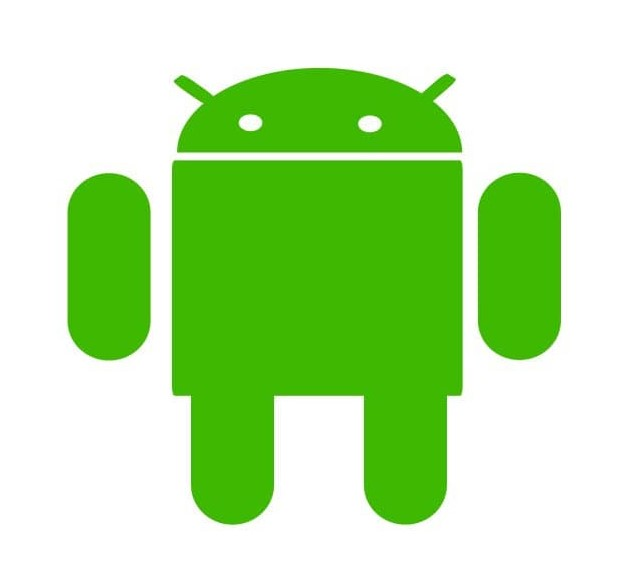
\includegraphics[width=0.2\linewidth]{res/Android.jpg}}
\subfigure[Logo Apple-a]{
\includegraphics[width=0.28\linewidth]{res/Apple.jpg}}
\subfigure[Logo iOS-a]{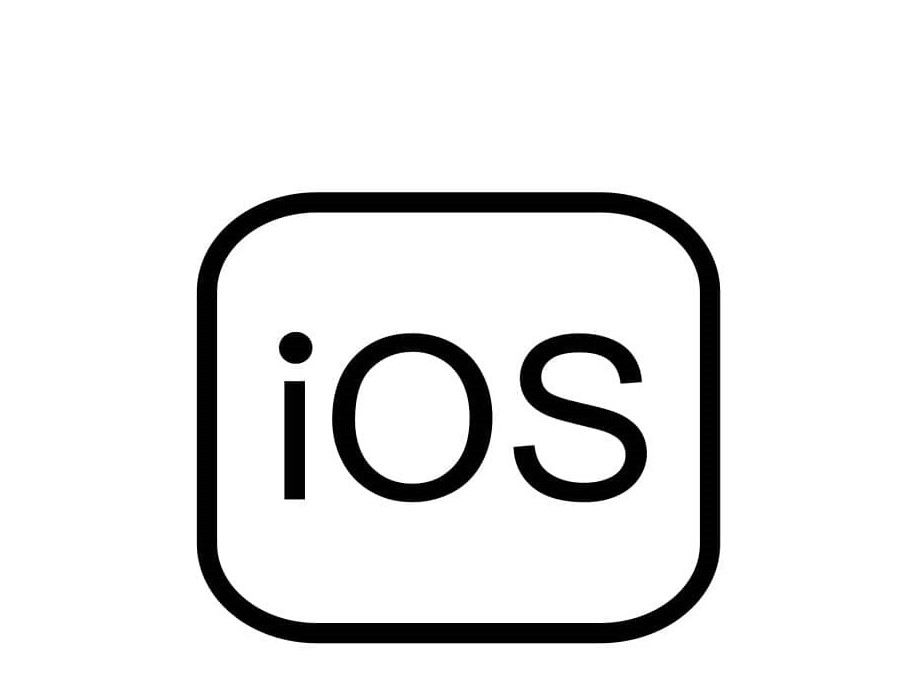
\includegraphics[width=0.3\linewidth]{res/iOS.jpg}}
\caption{Izgledi logo-a}
\label{fig: RIM BlackBerry}
\end{figure}
\end{frame}
\section{Historija}
\subsection{Historija Androida}
\begin{frame}{Historija Androida}
\begin{itemize}
\item Android je kreirao Andy Rubin 2003. godine
\item 2005. Google kupuje Android.inc
\item HTC postaje kompanija koja na tržište izbacuje mobilni uredjaj sa Android operativnim sistemom (HTC Dream)
\end{itemize}
\begin{figure}[h]
\centering
\captionsetup{}
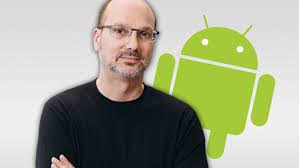
\includegraphics[width=0.65\columnwidth]{res/Andy.jpg}
\caption{Andy Rubin tvorac Androida}
\end{figure}
\end{frame}
\subsection{Historija iOS-a}
\begin{frame}{Historija iOS-a}
\begin{itemize}
\item Planiranje o stvaranju iPhona započinje 2005.
\item Forstallova pobjeda dovodi do stvaranja iOS-a
\item Prvi uredjaj je pušten u prodaju 2007.
\end{itemize}
\begin{figure}
\centering
\captionsetup{}
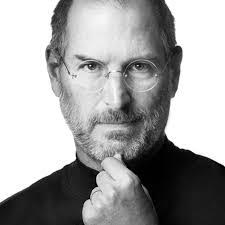
\includegraphics[width=0.45\columnwidth]{res/jobs.jpg}
\caption{Steve Jobs}
\end{figure}
\end{frame}
\section{Android vs iOS}
\subsection{Prednosti Androida}
\begin{frame}{Prednosti Androida}
\begin{itemize}
\item Poboljšana sigurnost i privatnost aplikacija
\item Poboljšana komunikacija
\item Snimanje ekrana
\item Veliki hardverski izbori
\item Podrška za 5g mreže
\end{itemize}
\begin{figure}
\centering
\captionsetup{}
\includegraphics[width=0.4\columnwidth]{res/inter.jpg}
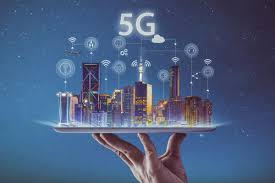
\includegraphics[width=0.4\columnwidth]{res/5g.jpg}
\caption{Android 5g}
\end{figure}
\end{frame}
\subsection{Prednosti iOS-a}
\begin{frame}{Prednosti iOS-a}
\begin{itemize}
\item Bolja organizacija ikona aplikacije 
\item Obavijesti su manje nametljive
\item Bolje i jasnije mape(navigacija)
\item Mogućnost odabira defaultnih aplikacija web preglednika
\end{itemize}
\begin{figure}[h]
\centering
\captionsetup{}
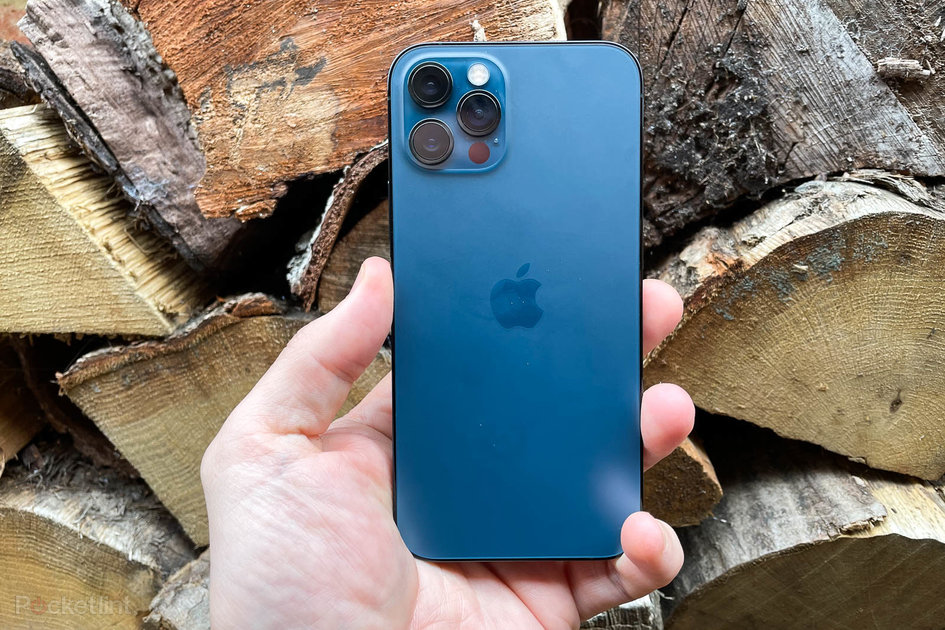
\includegraphics[width=0.55\columnwidth]{res/iphone.jpg}
\caption{iPhone}
\end{figure}
\end{frame}
\subsection{Nedostaci Androida}
\begin{frame}{Nedostaci Androida}
\begin{itemize}
\item Većina trenutnih Androida neće dobiti novu verziju
\item Postojanje određena složenost i nedosljednost u odnosu na iOS
\item Slabija povezanost sa desktop i nosivim ekosistemom nego što je to slučaj kod iOS-a
\end{itemize}
\end{frame}
\subsection{Nedostaci iOS-a}
\begin{frame}{Nedostaci iOS-a}
\begin{itemize}
\item Nekoliko nezavisnih aplikacija ažurirano je za nove kao što je App clips i widgeti
\item Mali broj jezika u aplikaciji Prevoditelj
\item Carkey ima ograničenu kompatiblnost vozila
\end{itemize}
\end{frame}
\section{Hardver}
\begin{frame}{Hardver}
\begin{itemize}
\item iOS nema veliki izbor proizvoda jer je Closed-source tipa
\item Android ima mnogo već izbor jer je Open-source tipa
\item Android je znatno jeftinija opcija za prosječnog korisnika 
\end{itemize}
\begin{figure}[h]
\centering
\captionsetup{}
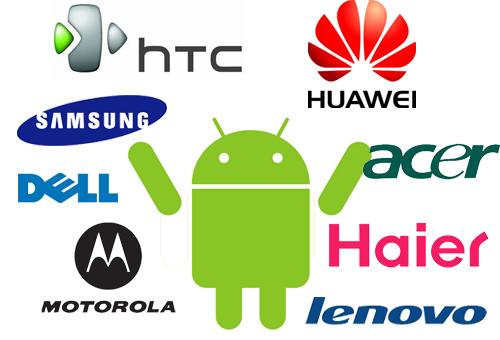
\includegraphics[width=0.65\columnwidth]{res/hardver.jpg}
\caption{Kompanije koje koriste android}
\end{figure}
\end{frame}
\section{Interfejs}
\begin{frame}{Interfejs}
\begin{itemize}
\item Andriod ima slobodniji interfejs dok je iOS striktniji u tom pogledu
\item iOS 14- najnovija verzija omogućava prilagodbu korisnika
\end{itemize}
\begin{figure}[h]
\centering
\captionsetup{}
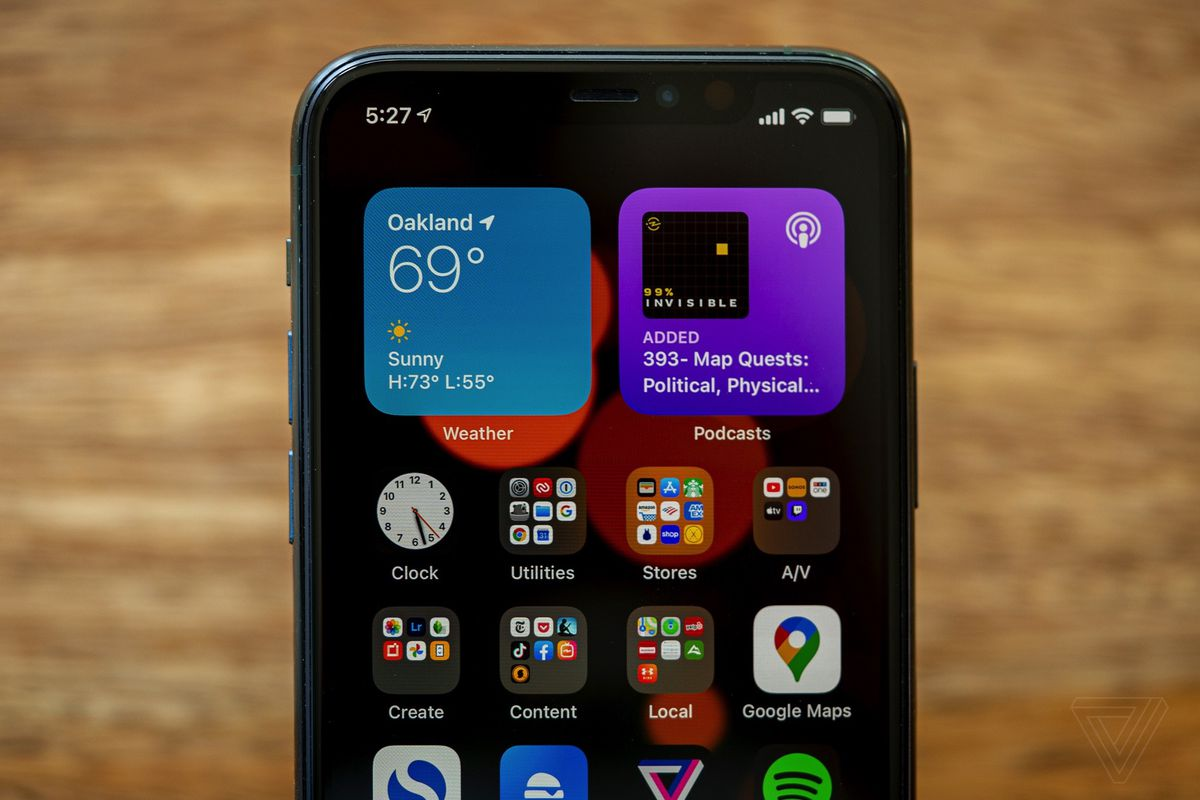
\includegraphics[width=0.65\columnwidth]{res/iphone14.jpg}
\caption{Interfejs na iOS 14}
\end{figure}
\end{frame}
\section{Uključene aplikacije}
\begin{frame}{Uključene aplikacije}
\begin{itemize}
\item U ponudi veliki broj aplikacija
\item Jedna od značajnijih je mapiranje
\item Oba operativan sistema nude izvrsne aplikacije (nadzor zdravlja, vijesti, podcast...)
\end{itemize}
\begin{figure}[h]
\centering
\captionsetup{}
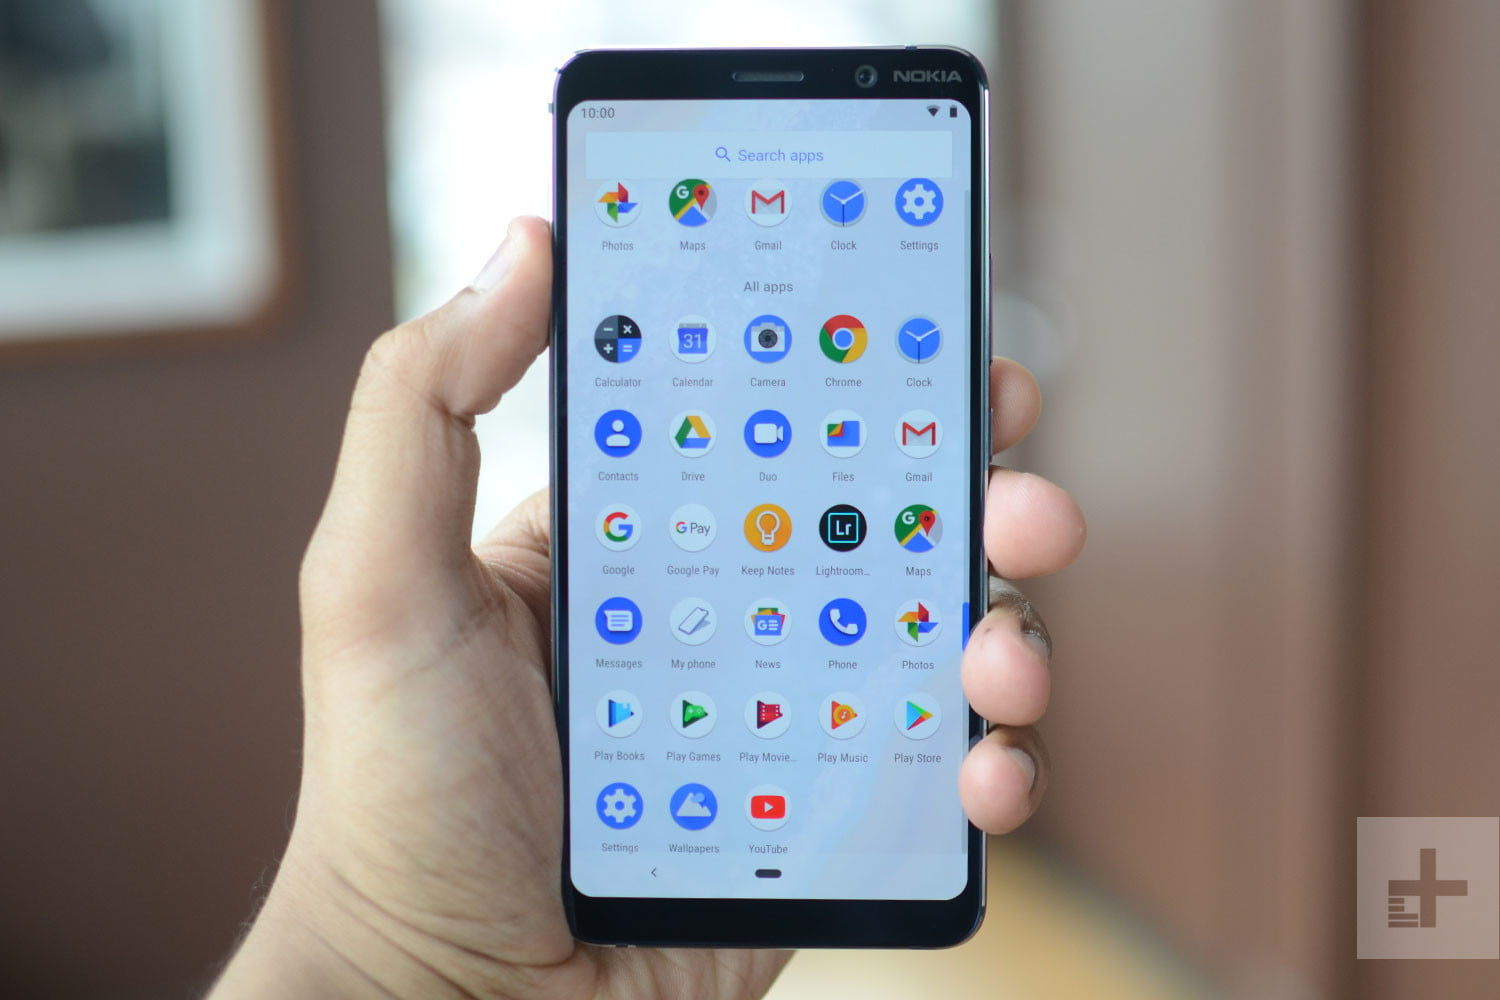
\includegraphics[width=0.65\columnwidth]{res/Ukljucene.jpg}
\caption{Stock aplikacije na Androidu}
\end{figure}
\end{frame}
\section{Ekosistem aplikacije}
\begin{frame}{Ekosistem aplikacije}
\begin{itemize}
\item Android ima opciju za instaliranje aplikacija izvan Google trgovine
\item Mogućnost daljinskog instaliranja aplikacija
\end{itemize}
\begin{figure}[h]
\centering
\captionsetup{}
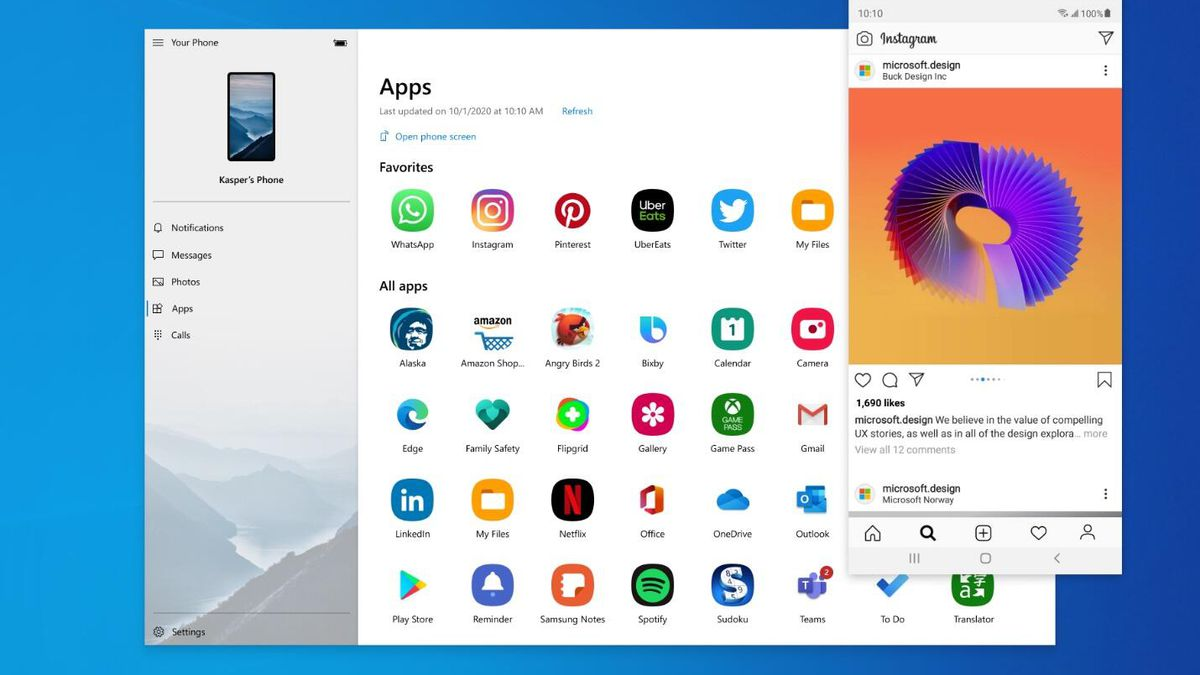
\includegraphics[width=0.65\columnwidth]{res/Ekosistem.jpg}
\caption{Instalacija aplikacija pomoću laptopa}
\end{figure}
\end{frame}
\section{Igre, VR i AR}
\begin{frame}{Igre, VR i AR}
\begin{itemize}
\item Velike biblioteke igara približno razini konzola
\item Mogućnost pretplate
\item iOS nudi veći izbor VR aplikacija
\end{itemize}
\begin{figure}[h]
\centering
\captionsetup{}
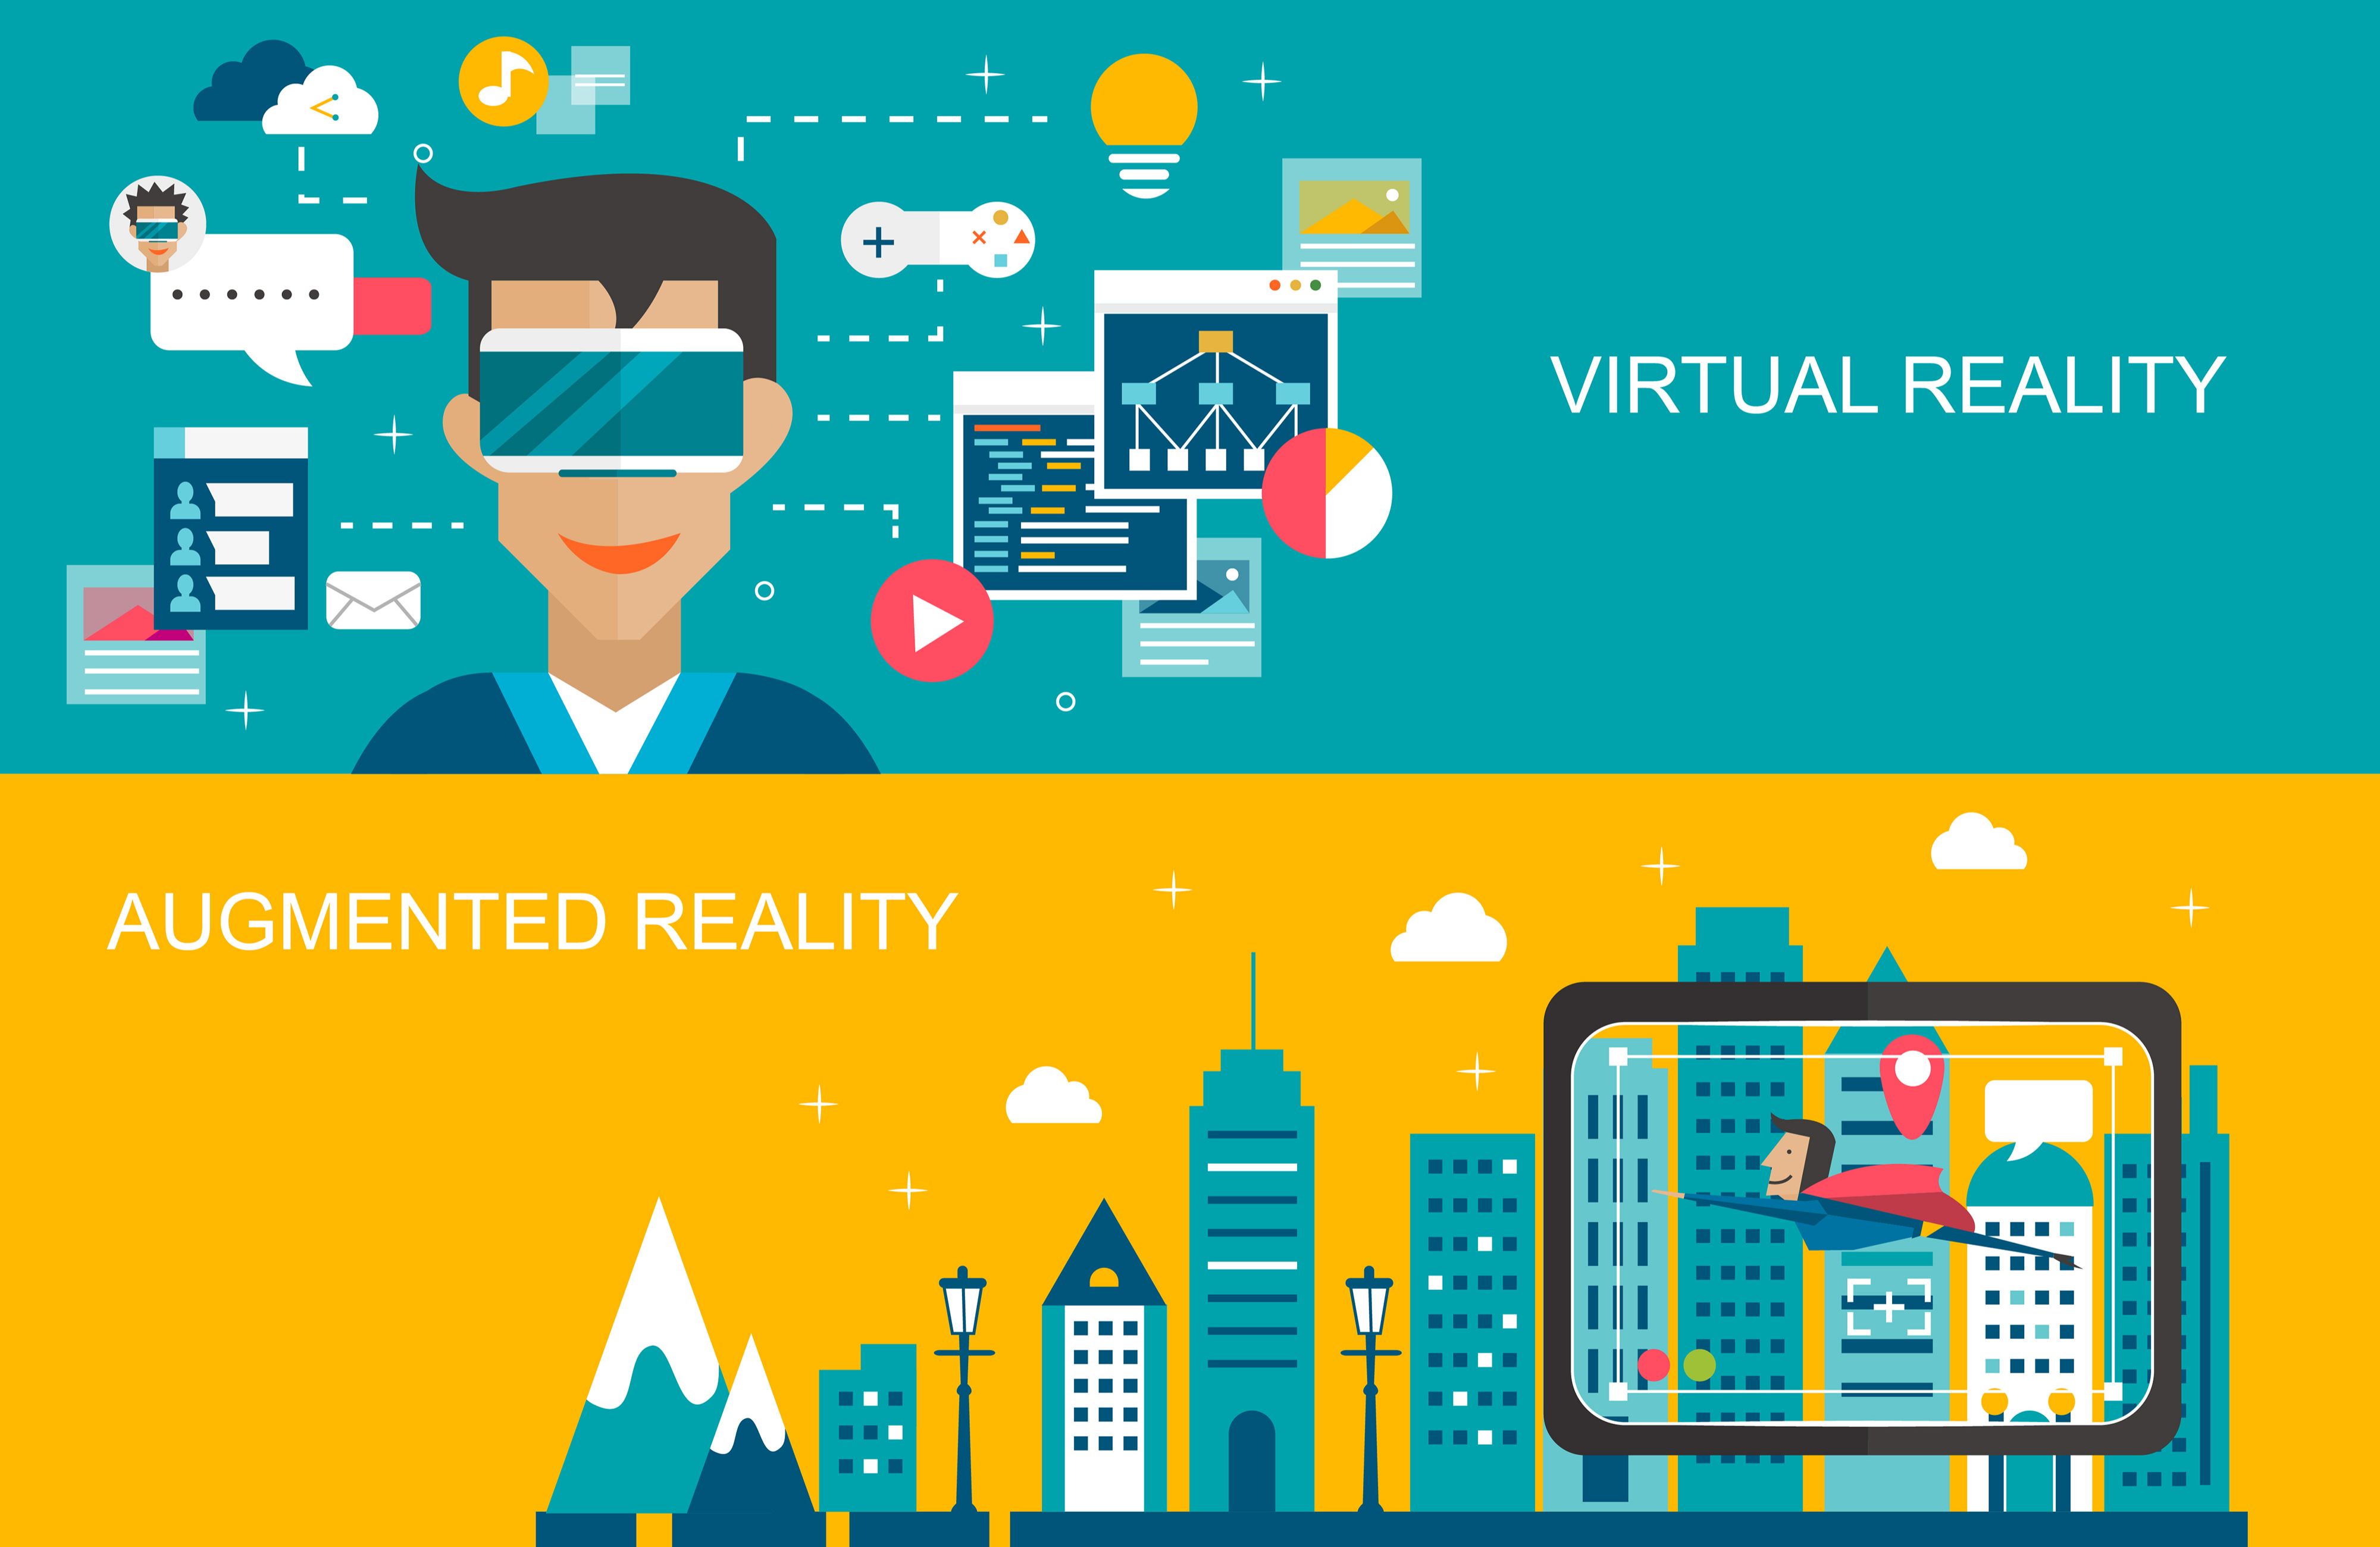
\includegraphics[width=0.65\columnwidth]{res/AR_VR.jpg}
\caption{Razlika izmedju AR i VR}
\end{figure}
\end{frame}
\section{Kamere i fotografije}
\begin{frame}{Kamere i fotografije}
\begin{itemize}
\item Kamere u fokusu novih izdanja smartphone-a
\item Impresivan softver za poboljšanje fotografije
\item Kompanija Huawei se istekla sa night modom
\end{itemize}
\begin{figure}[h]
\centering
\captionsetup{}
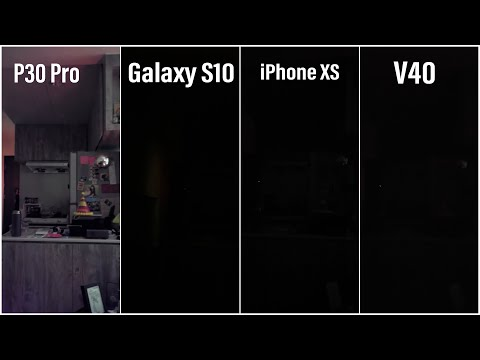
\includegraphics[width=0.65\columnwidth]{res/dark_mode.jpg}
\caption{Poredjenje dark-moda na različitim telefonima}
\end{figure}

\end{frame}
\section{Zaključak}
\begin{frame}{Zaključak}
\begin{itemize}
\item Nadamo se da smo uspjeli objasniti razlike izmedju Androida i iOS-a
\item Ne postoji najbolji operativni sistem, ali postoje razlike koje nam daju uvid u ono što želimo.
\item Možemo potvrditi da su oba operativna sistema kvalitetna, brza, responzivna i jednostavna za upotrebu.
\end{itemize}
\end{frame}

\end{document}